\section{Shape Sensitivity of Flow over a Cylinder}
% ==================================================
For the second demonstration problem, the flow over a cylinder is modeled using the virtual boundary method using Equation \eqref{eq:C4_NSwithvirtualBoundaryIB}. The sensitivity analysis is conducted by differentiating the NS equations as shown in Equation \eqref{eq:C4_NSwithvirtualBoundaryIBsensitivity}. For this problem the domain is defined as a rectangle with the cylinder located on the horizontal symmetry line as shown in Figure \ref{fig:C4_cylinderPhysicalDomain}.

\begin{figure}[H]
    \centering
    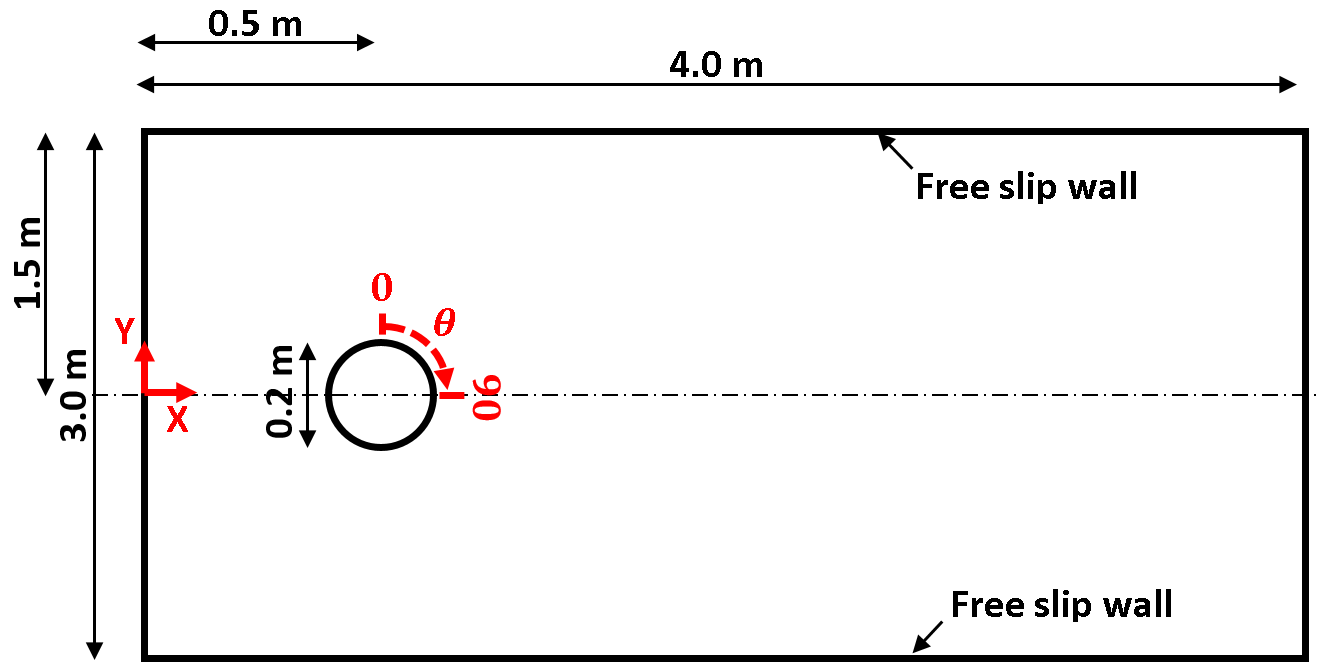
\includegraphics[width=12.00cm]{Chapter_4/figure/flow_over_cylinder/flow_over_cylinder.png}
    \caption{Physical domain with dimensions for flow over cylinder.}
    \label{fig:C4_cylinderPhysicalDomain}
\end{figure}

The boundary conditions are defined as the flow velocity at the inlet (left boundary) and the outflow (zero gradient) boundary condition at the outlet (right boundary). The top and bottom boundaries are modeled as free slip walls. The surface of the cylinder is modeled by the virtual boundary method. The mesh convergence for this problem for Reynolds number of 100 is shown in Figure \ref{fig:C4_meshConvergenceForCylidnerRE100GE}.

\begin{figure}[H]
    \centering
    \subfigure[U-velocity on y = 0.]
    {
    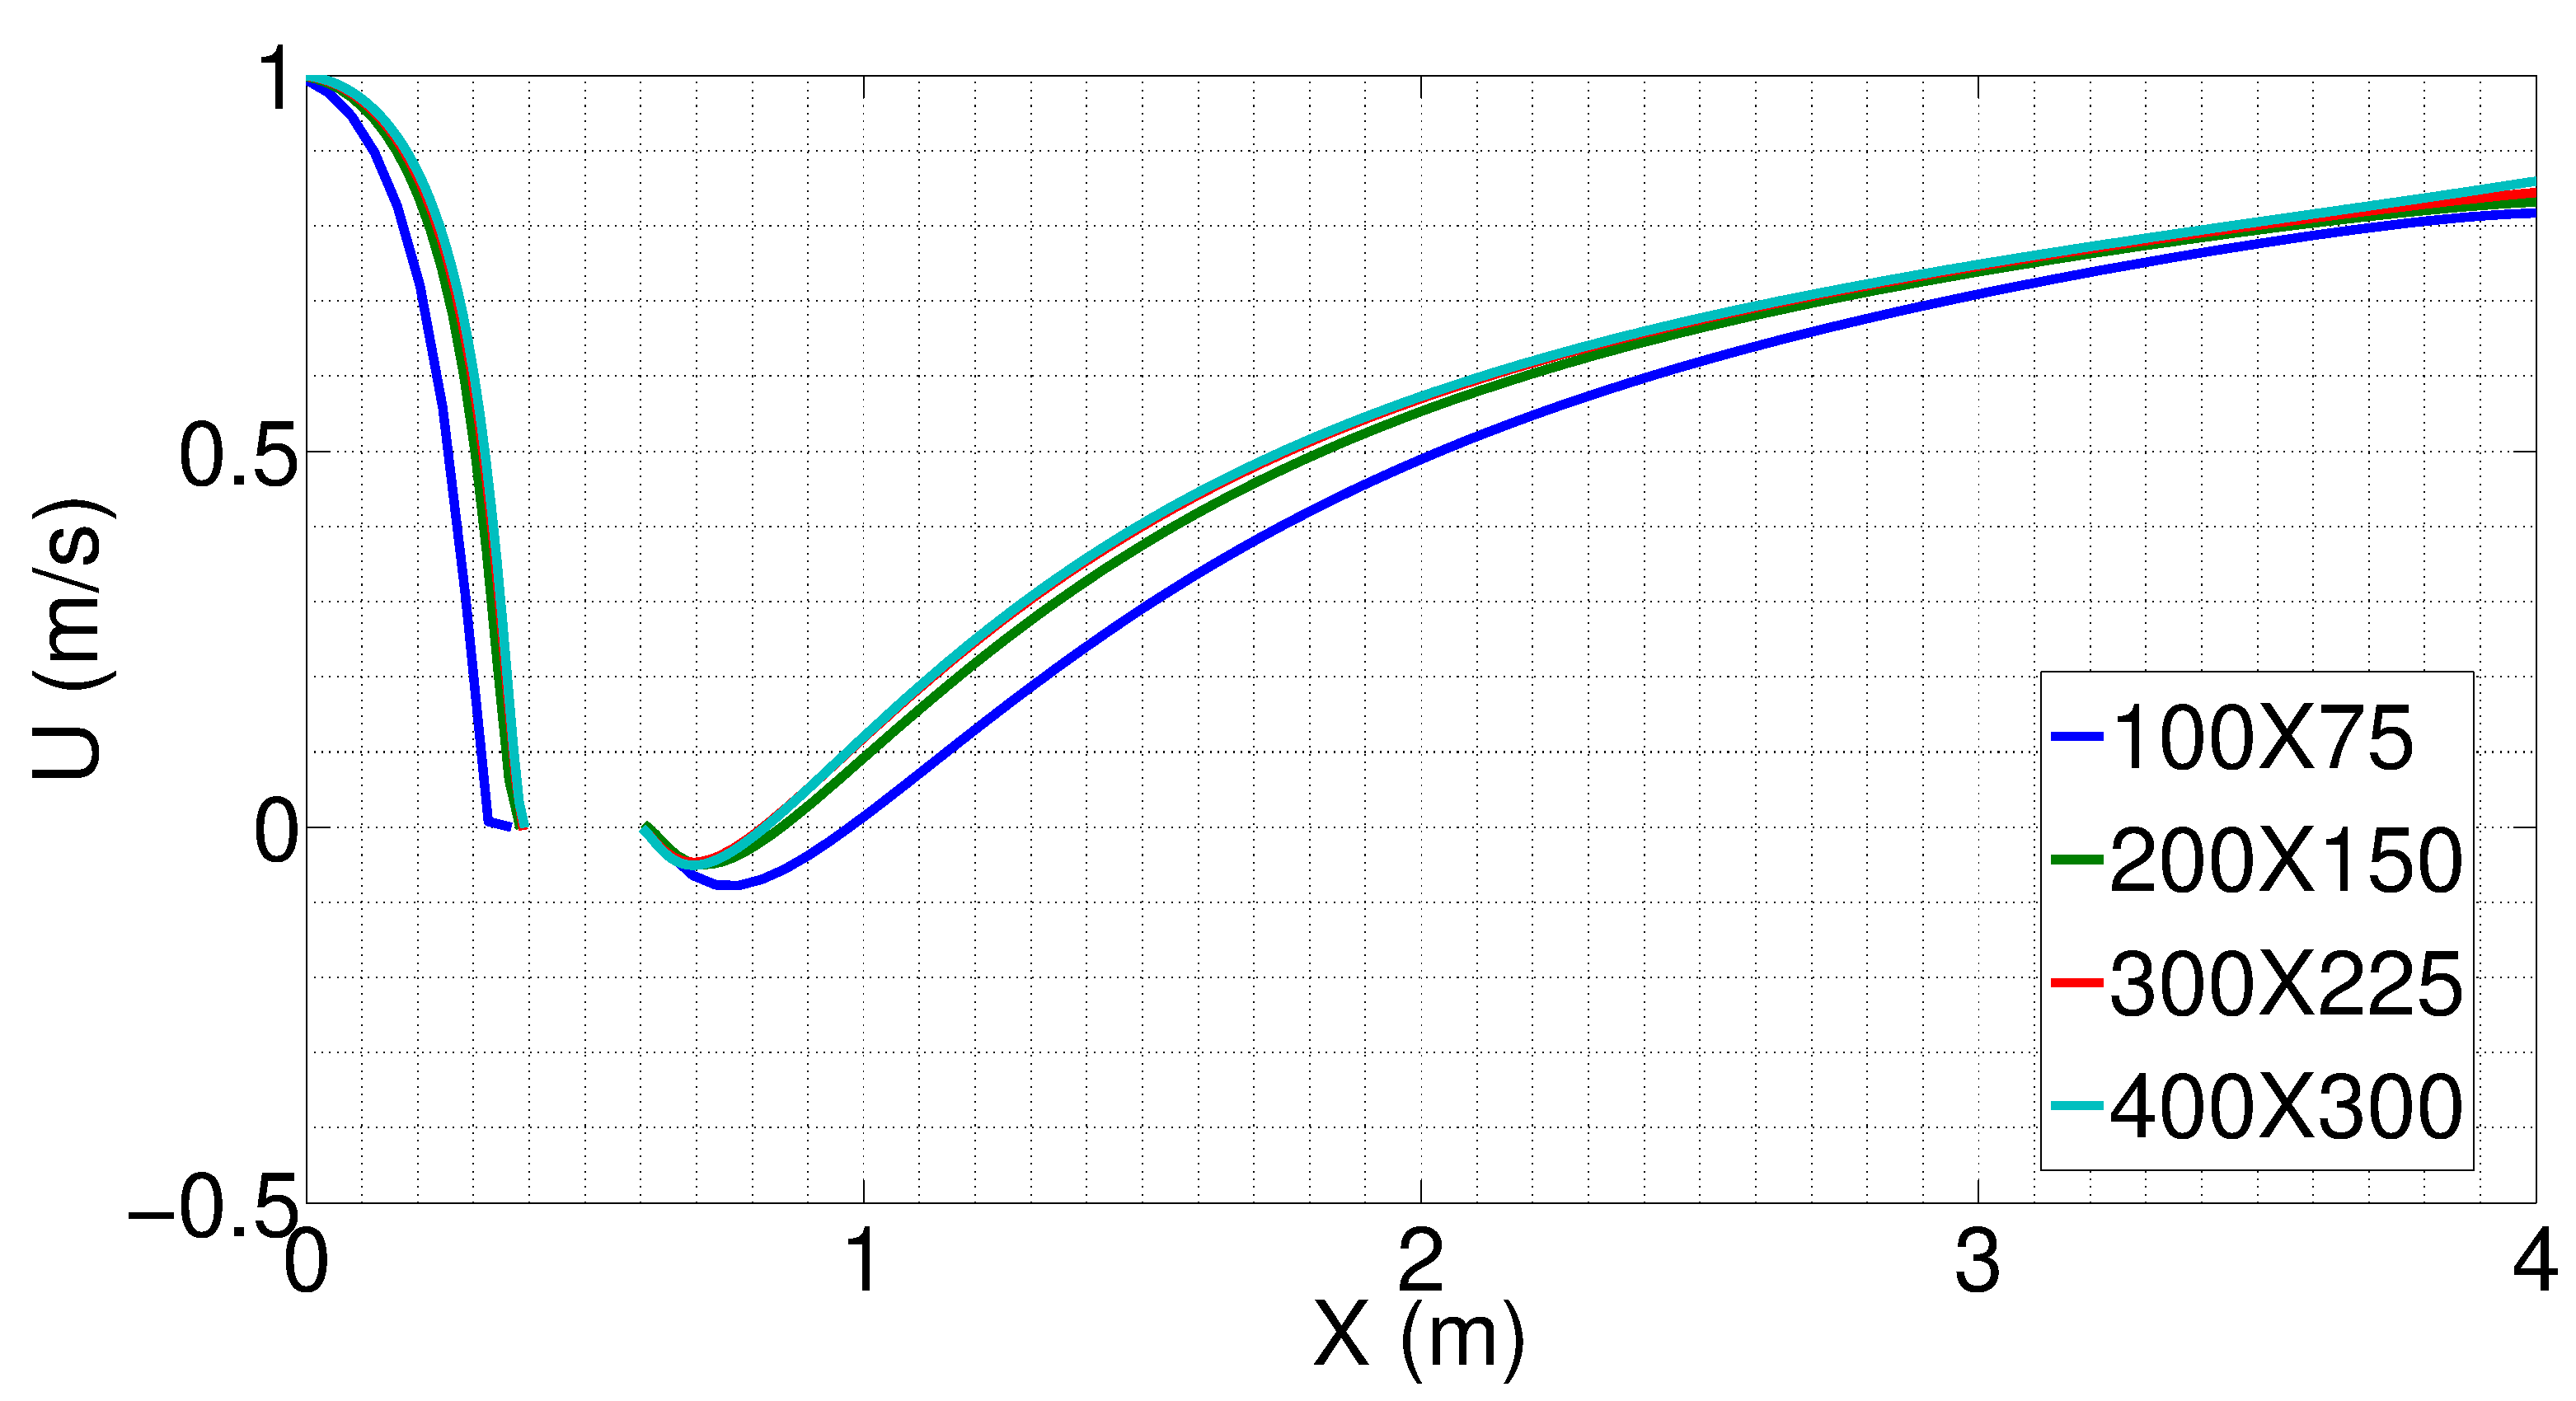
\includegraphics[width=7.0cm]{Chapter_4/figure/flow_over_cylinder/meshConvergence_RE100_U.eps}
    }
    \quad
    \subfigure[V-velocity on x = 0.5]
    {
    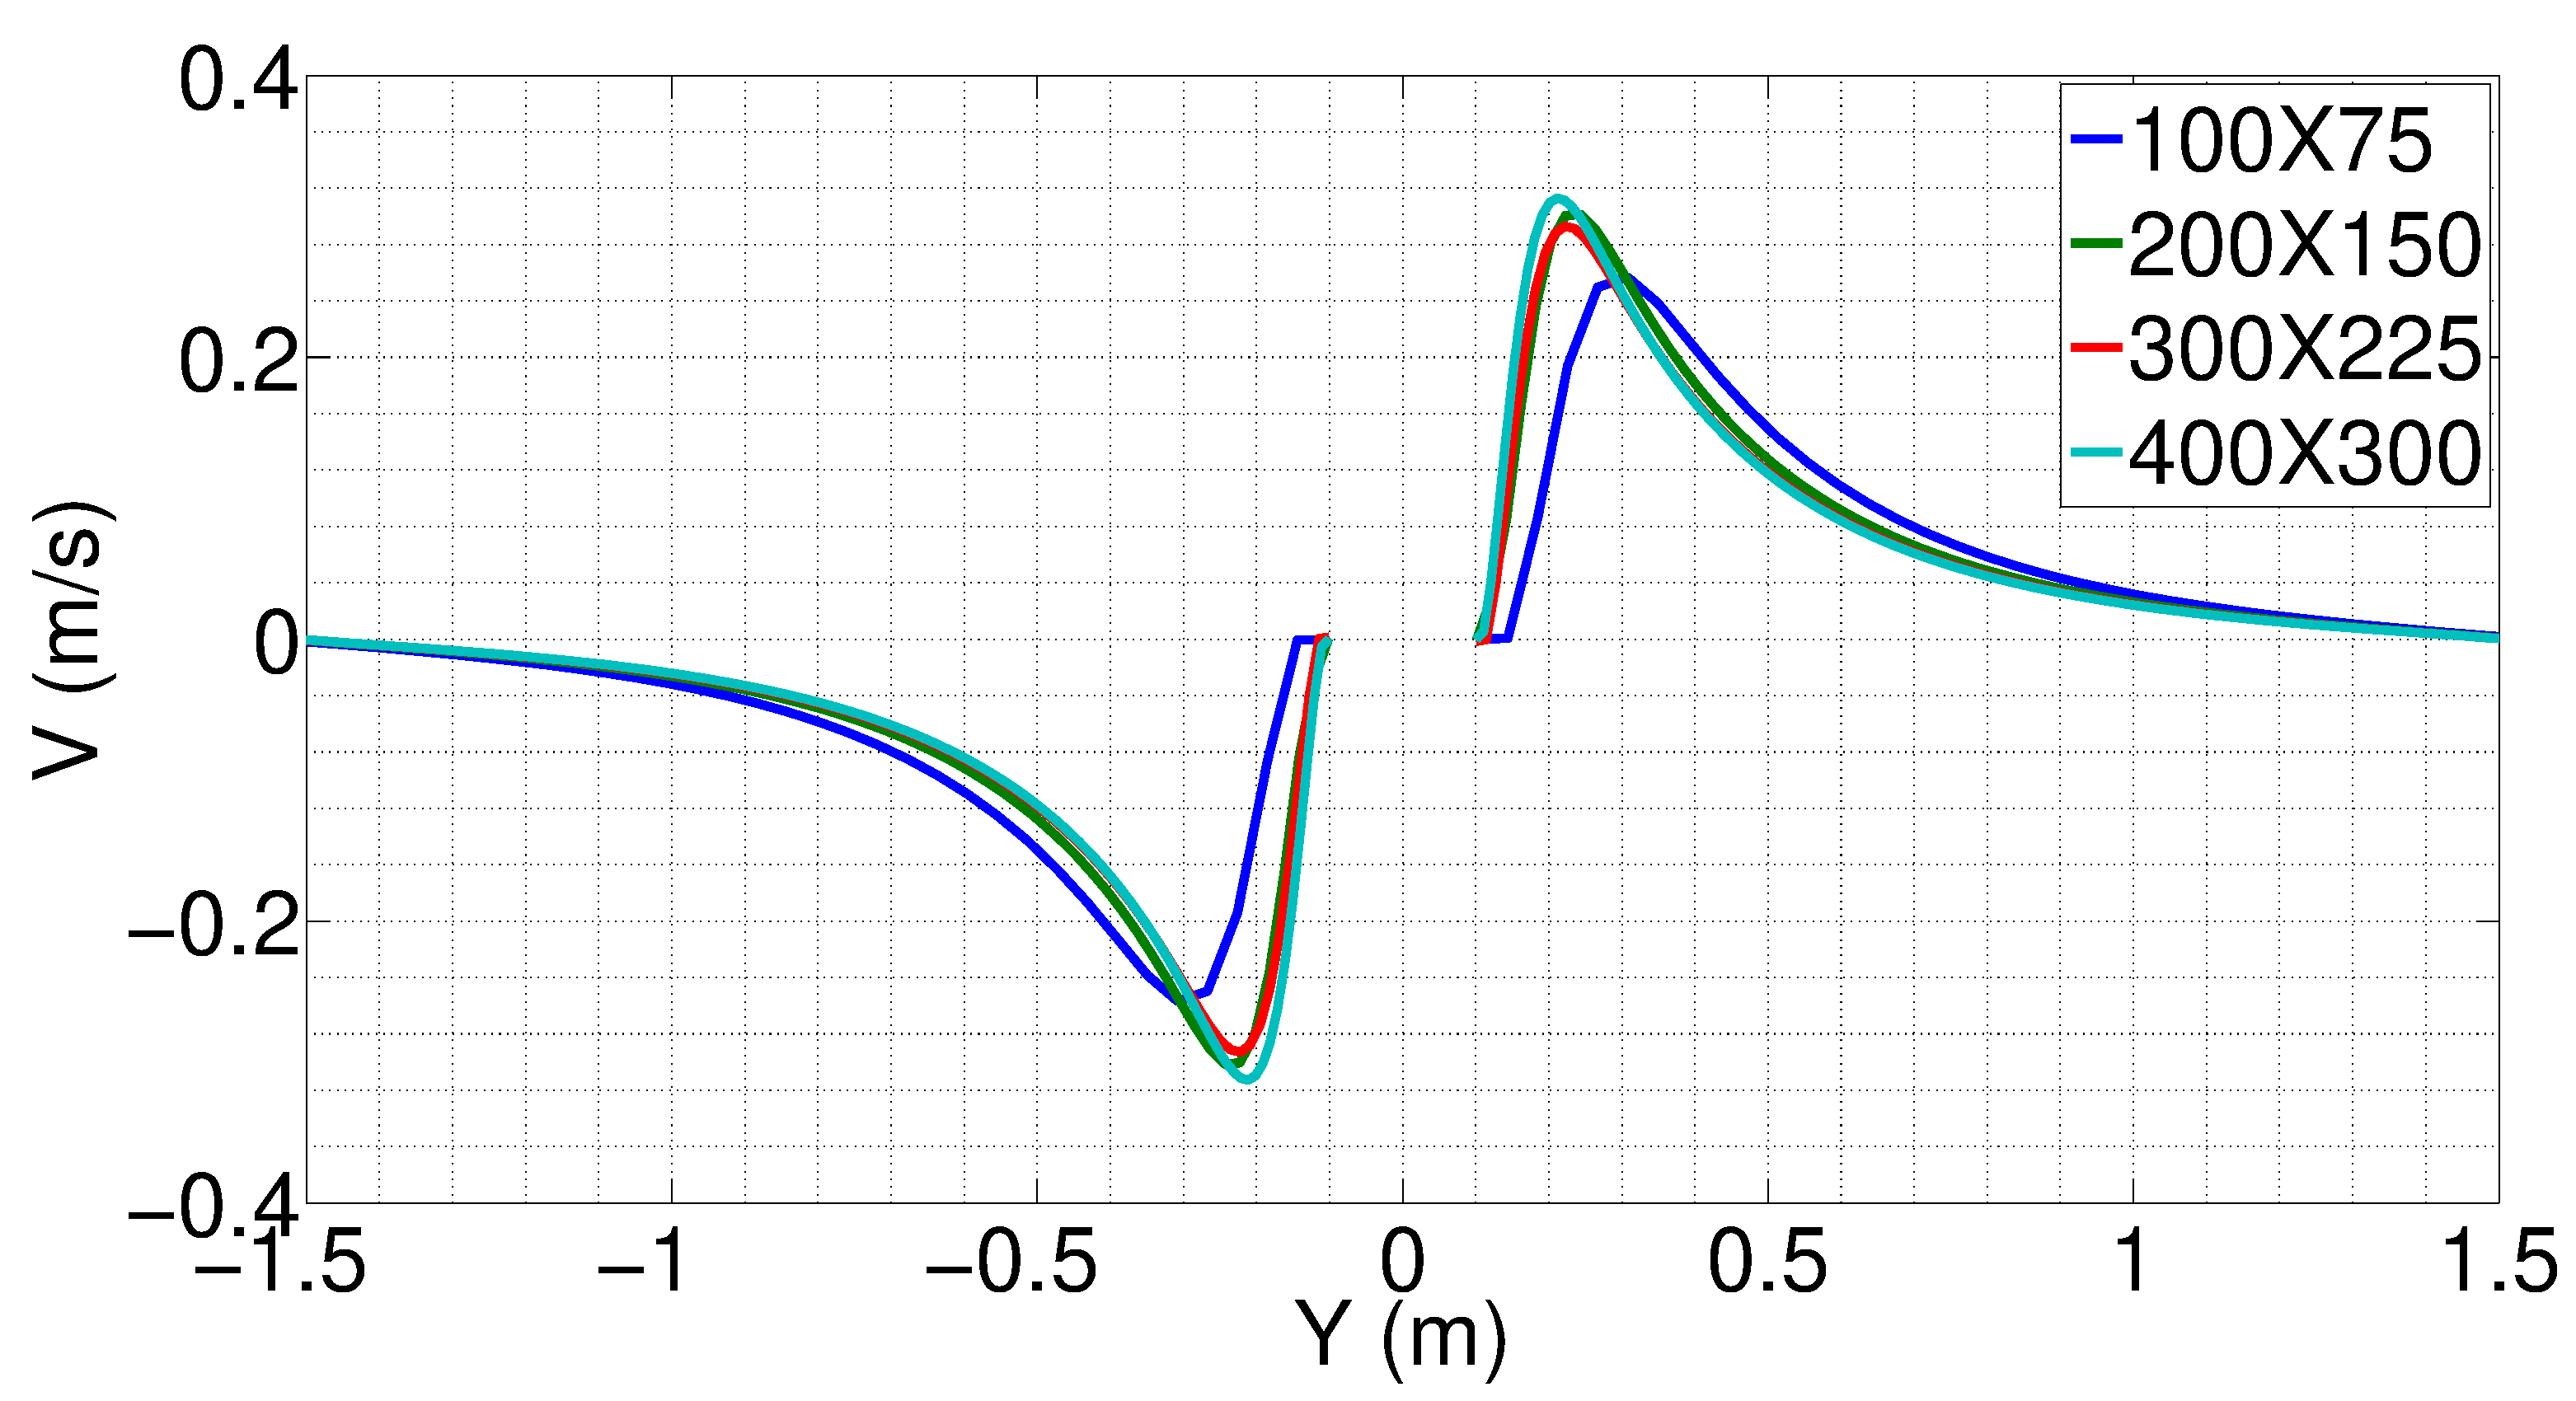
\includegraphics[width=7.0cm]{Chapter_4/figure/flow_over_cylinder/meshConvergence_RE100_V.eps}
    }
    \\
    \subfigure[Pressure on y = 0]
    {
    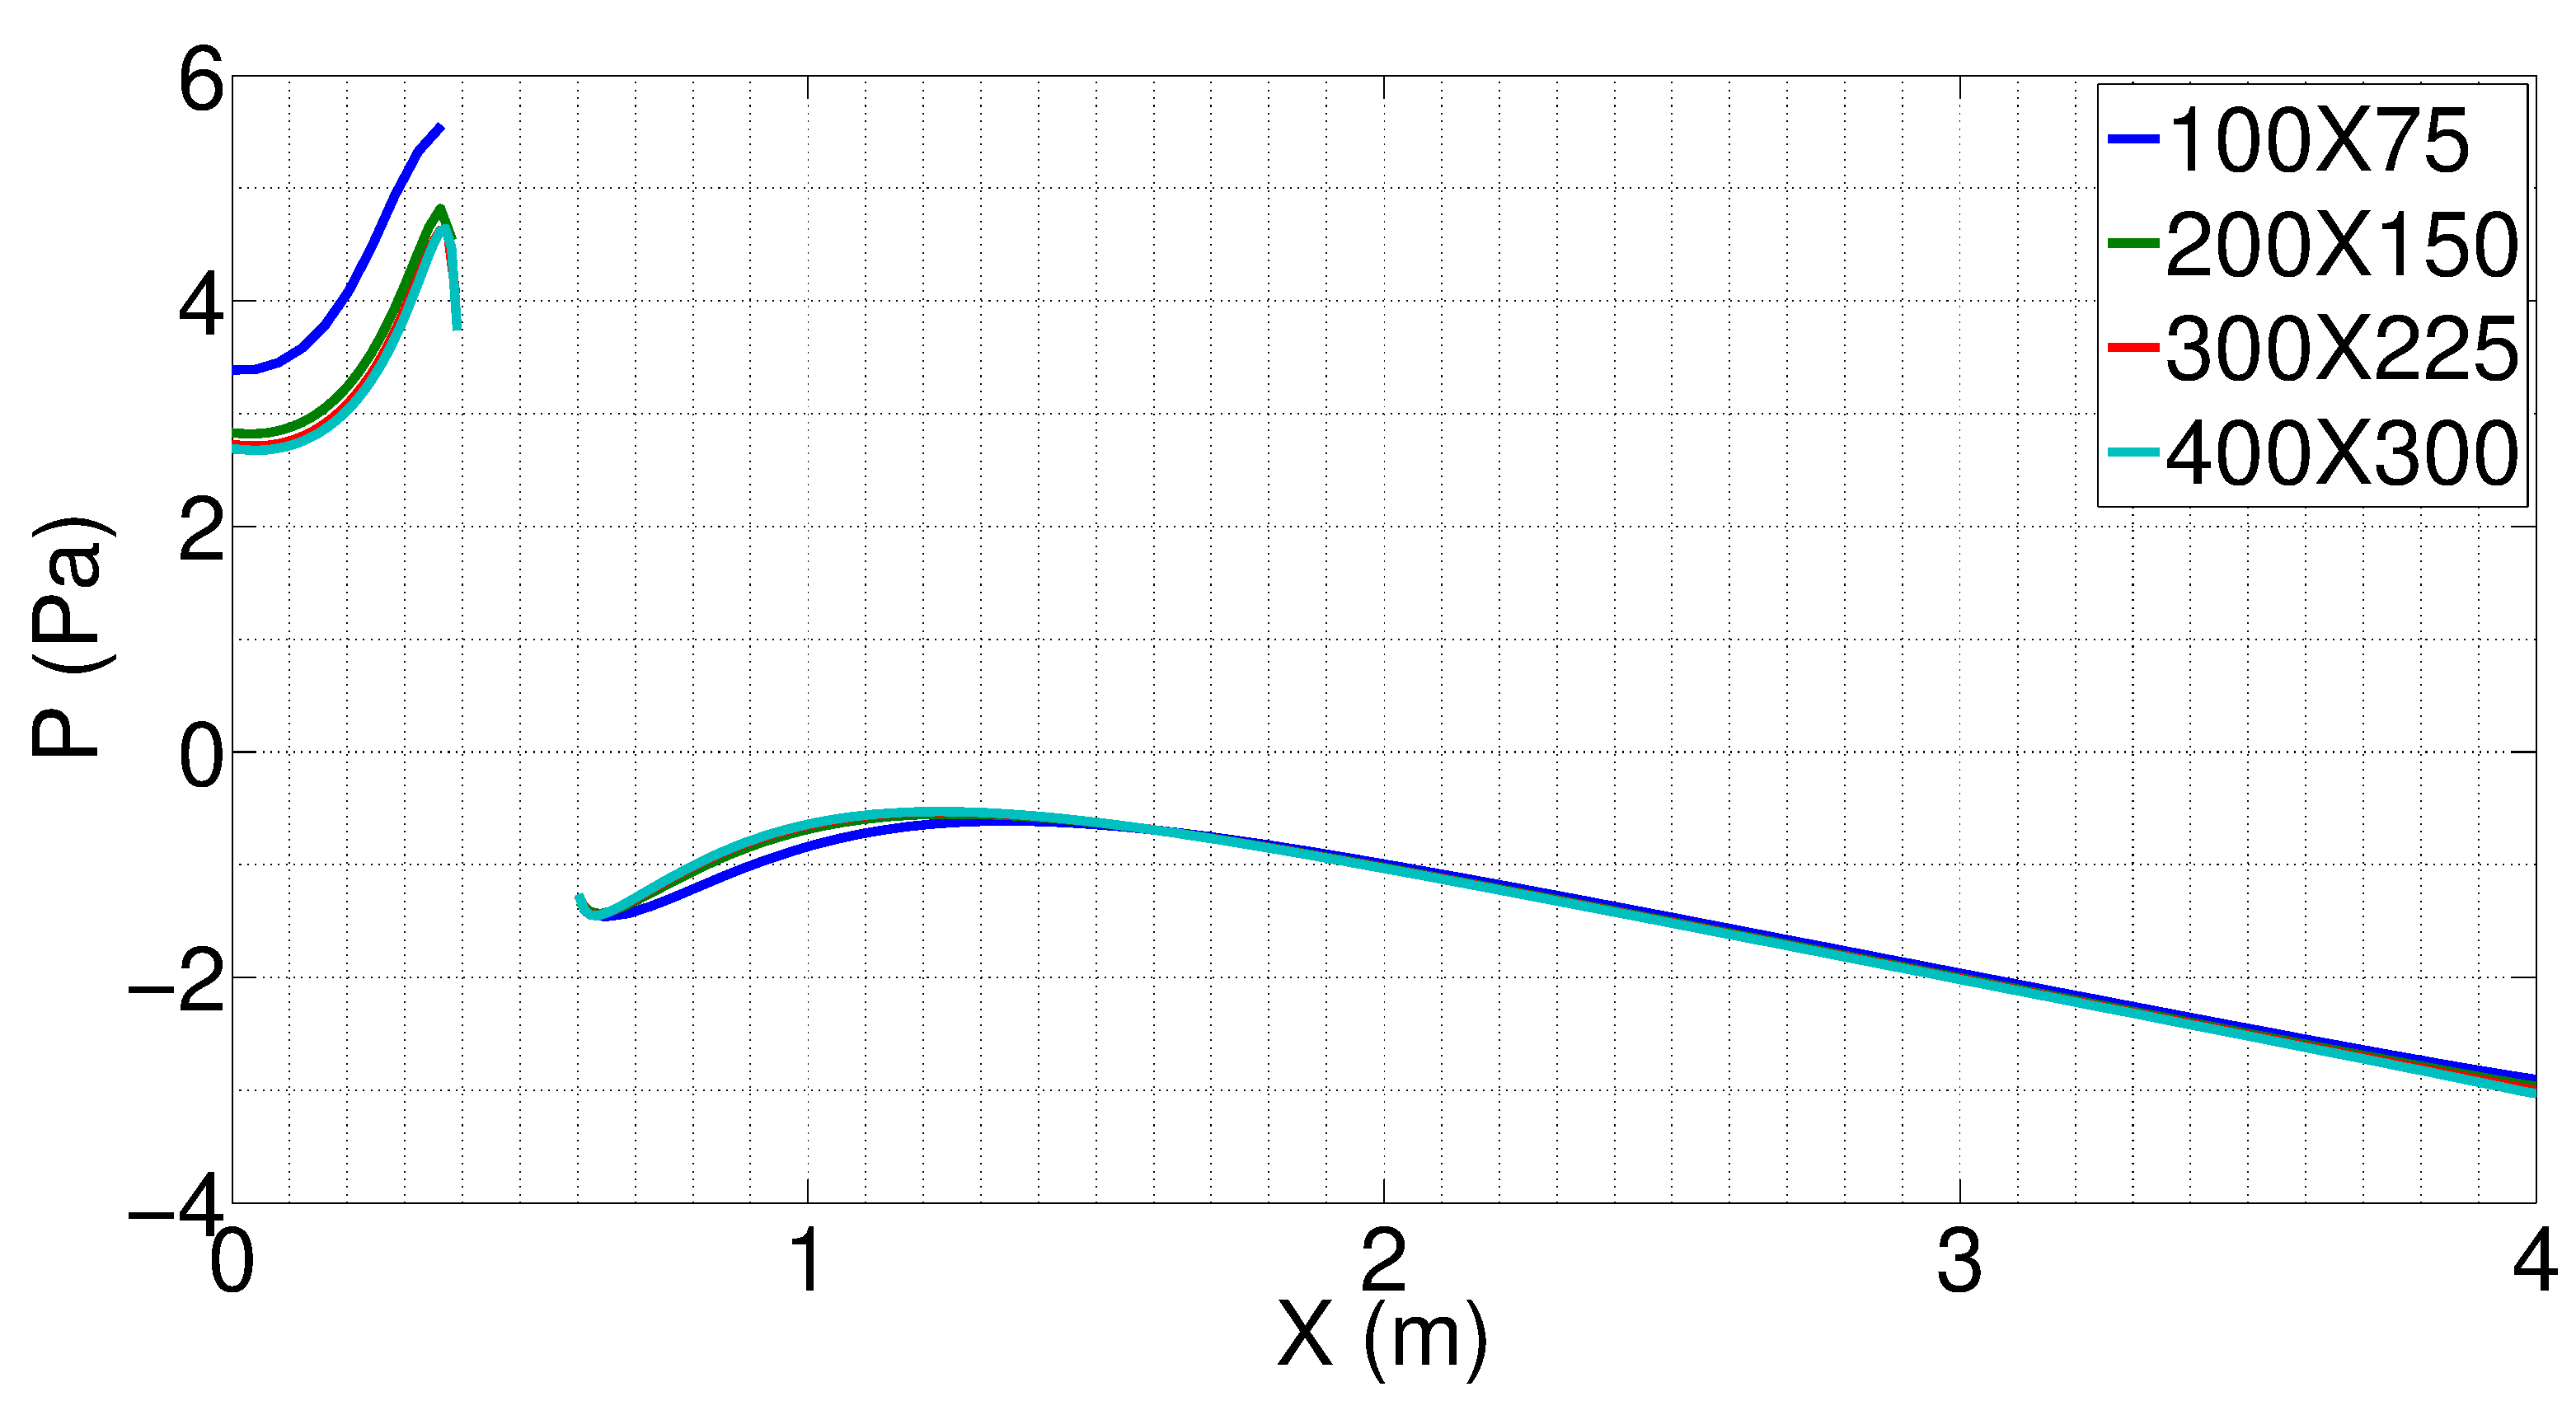
\includegraphics[width=7.0cm]{Chapter_4/figure/flow_over_cylinder/meshConvergence_RE100_P.eps}
    }
    \caption{Convergence results for Re = 100.}
    \label{fig:C4_meshConvergenceForCylidnerRE100GE}
\end{figure}

The convergence study of the mesh refinement is also conducted for a node on the downwash of the cylinder at $(2, 0)$ as shown in Figure \ref{fig:C4_meshRefinementForCylinderRE100GE}. The slopes of the fitted lines to the u-velocity, v-velocity, and pressure error estimates are calculated as $-2.34$, and $-1.96$, and $-2.72$. This means that the method is second order in space and time.

\begin{figure}[H]
    \centering
    \subfigure[U-velocity convergence on $(2.0, 0)$.]
    {
    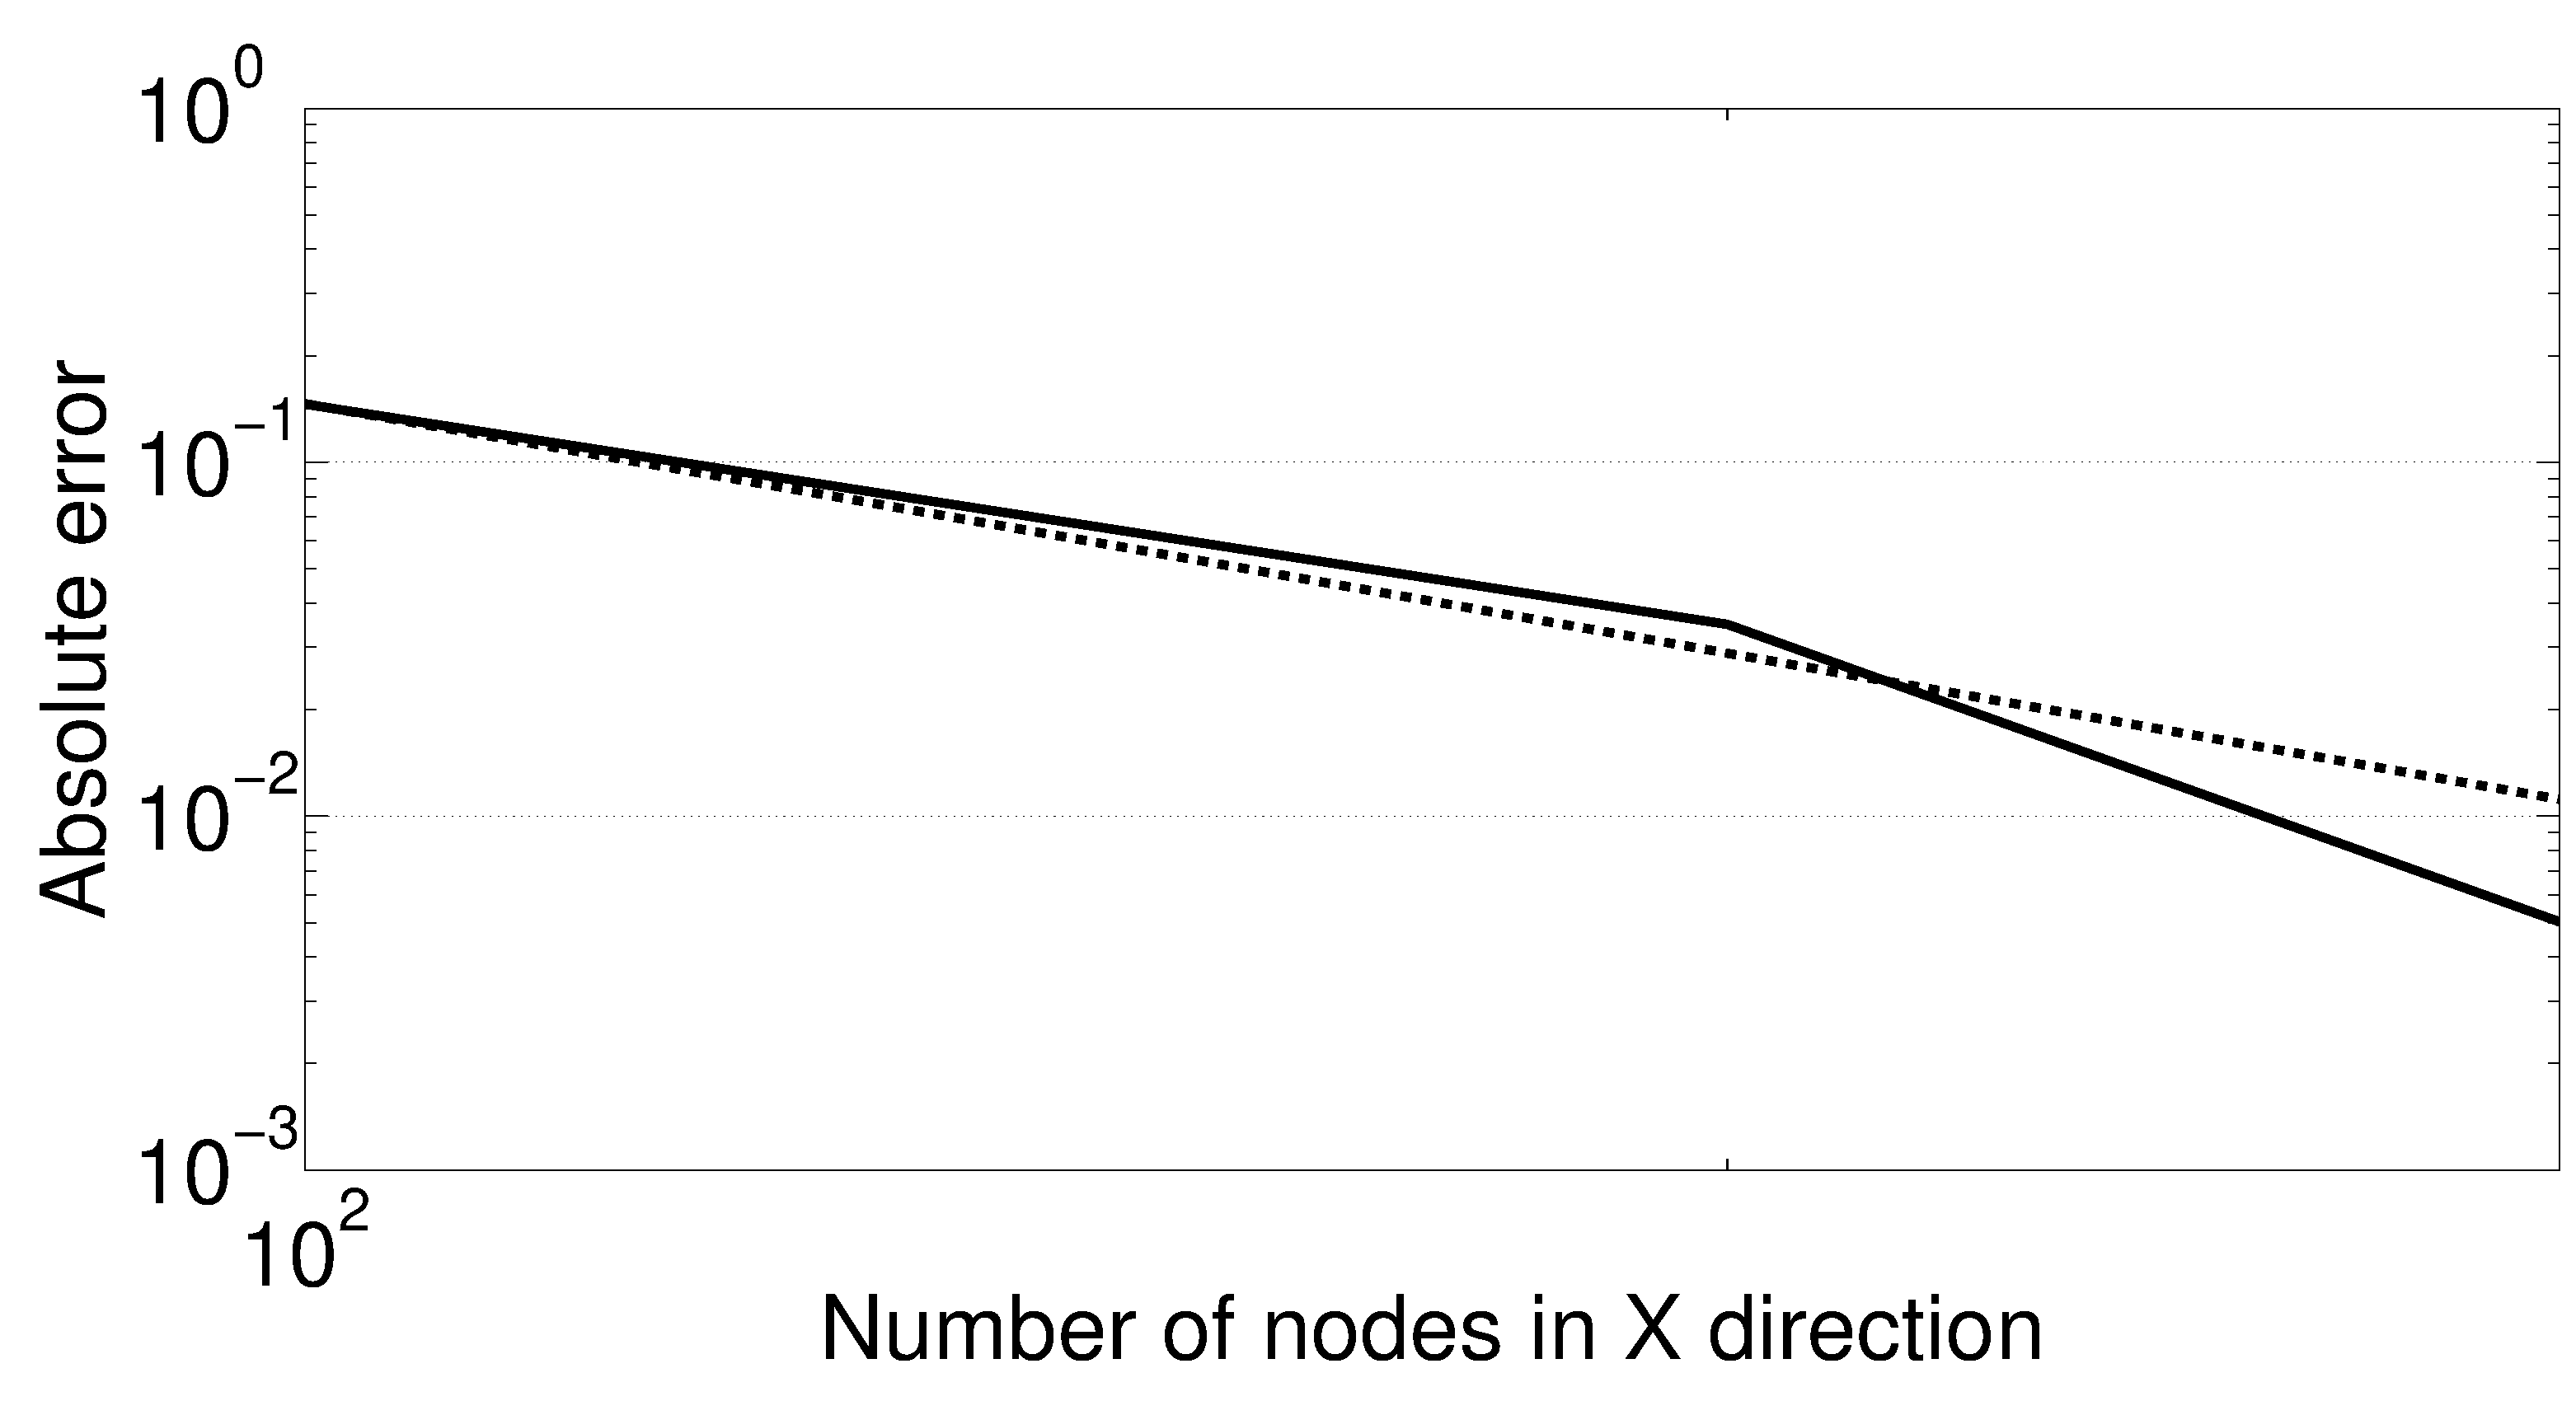
\includegraphics[width=7.0cm]{Chapter_4/figure/flow_over_cylinder/u_convergence_RE100.eps}
    }
    \quad
    \subfigure[V-velocity convergence on $(0.5, 0.75)$.]
    {
    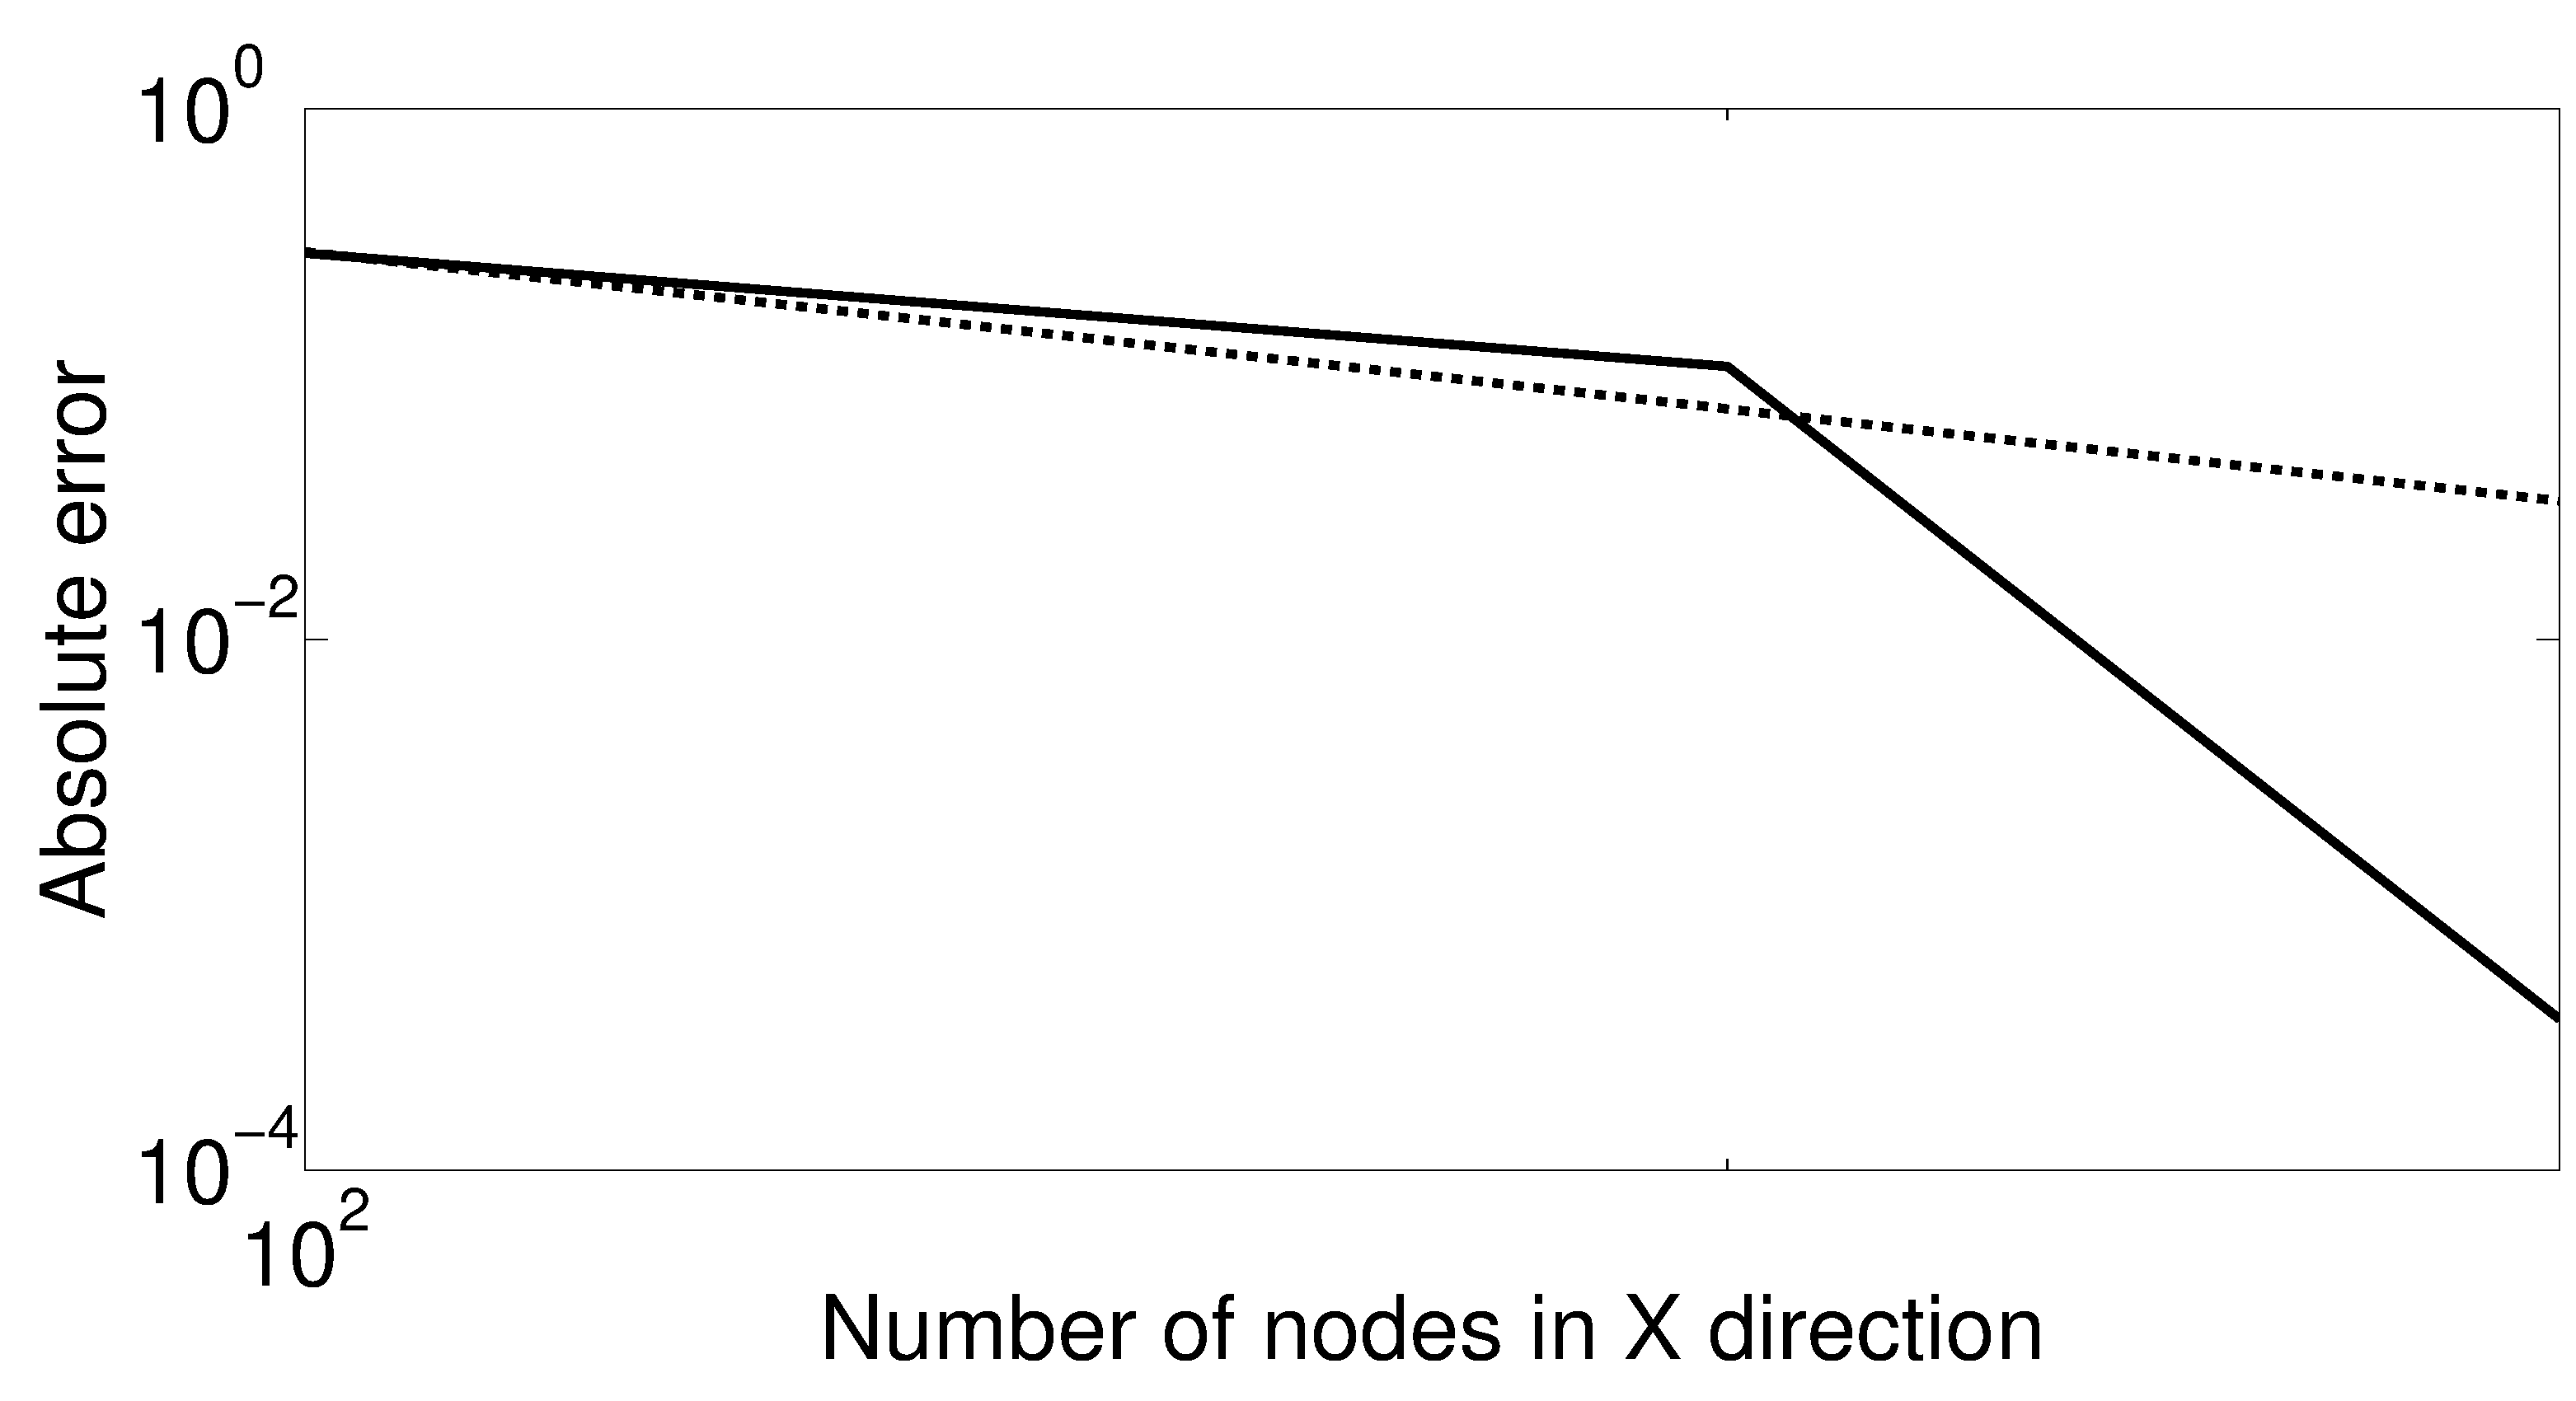
\includegraphics[width=7.0cm]{Chapter_4/figure/flow_over_cylinder/v_convergence_RE100.eps}
    }
    \\
    \subfigure[Pressure convergence on $(2.0, 0)$.]
    {
    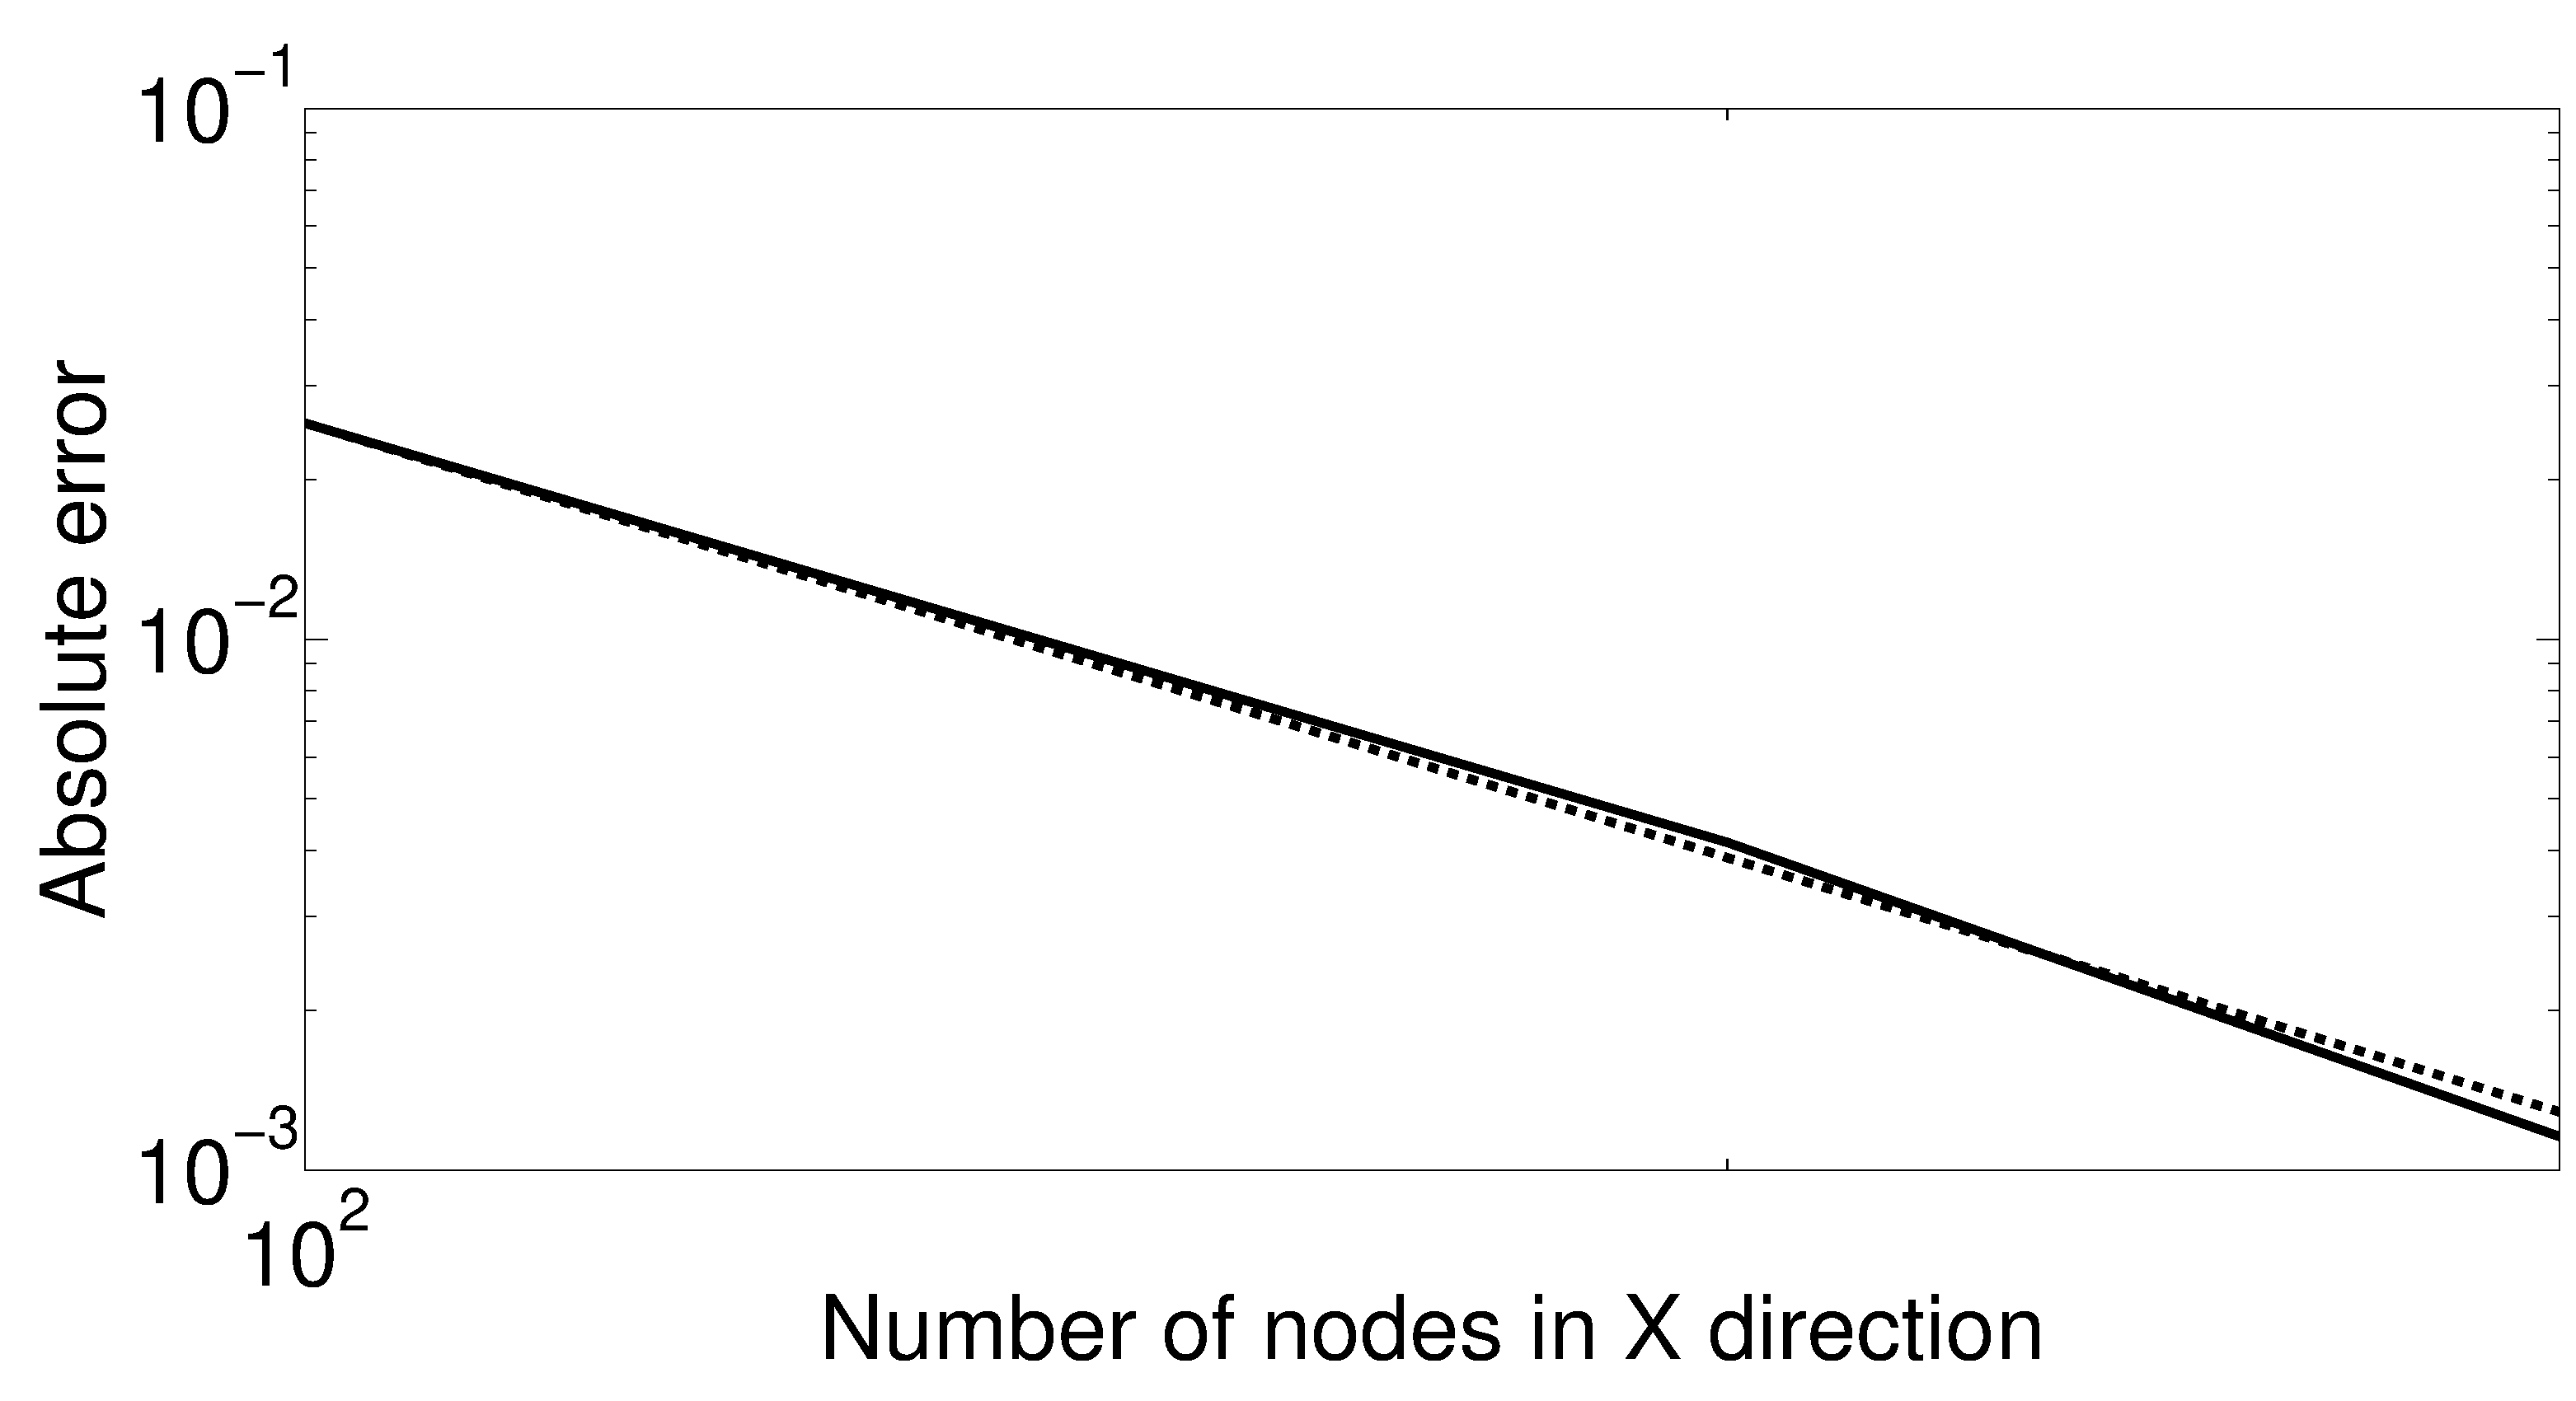
\includegraphics[width=7.0cm]{Chapter_4/figure/flow_over_cylinder/pressure_convergence_RE100.eps}
    }
    \caption{Convergence plots for Re = 100.}
    \label{fig:C4_meshRefinementForCylinderRE100GE}
\end{figure}

The contour plots for the velocity and pressure is shown in Figure \ref{fig:contourPlotsForFlowOverCylidnerGE}.

\begin{figure}[H]
    \centering
    \subfigure[U-velocity]
    {
    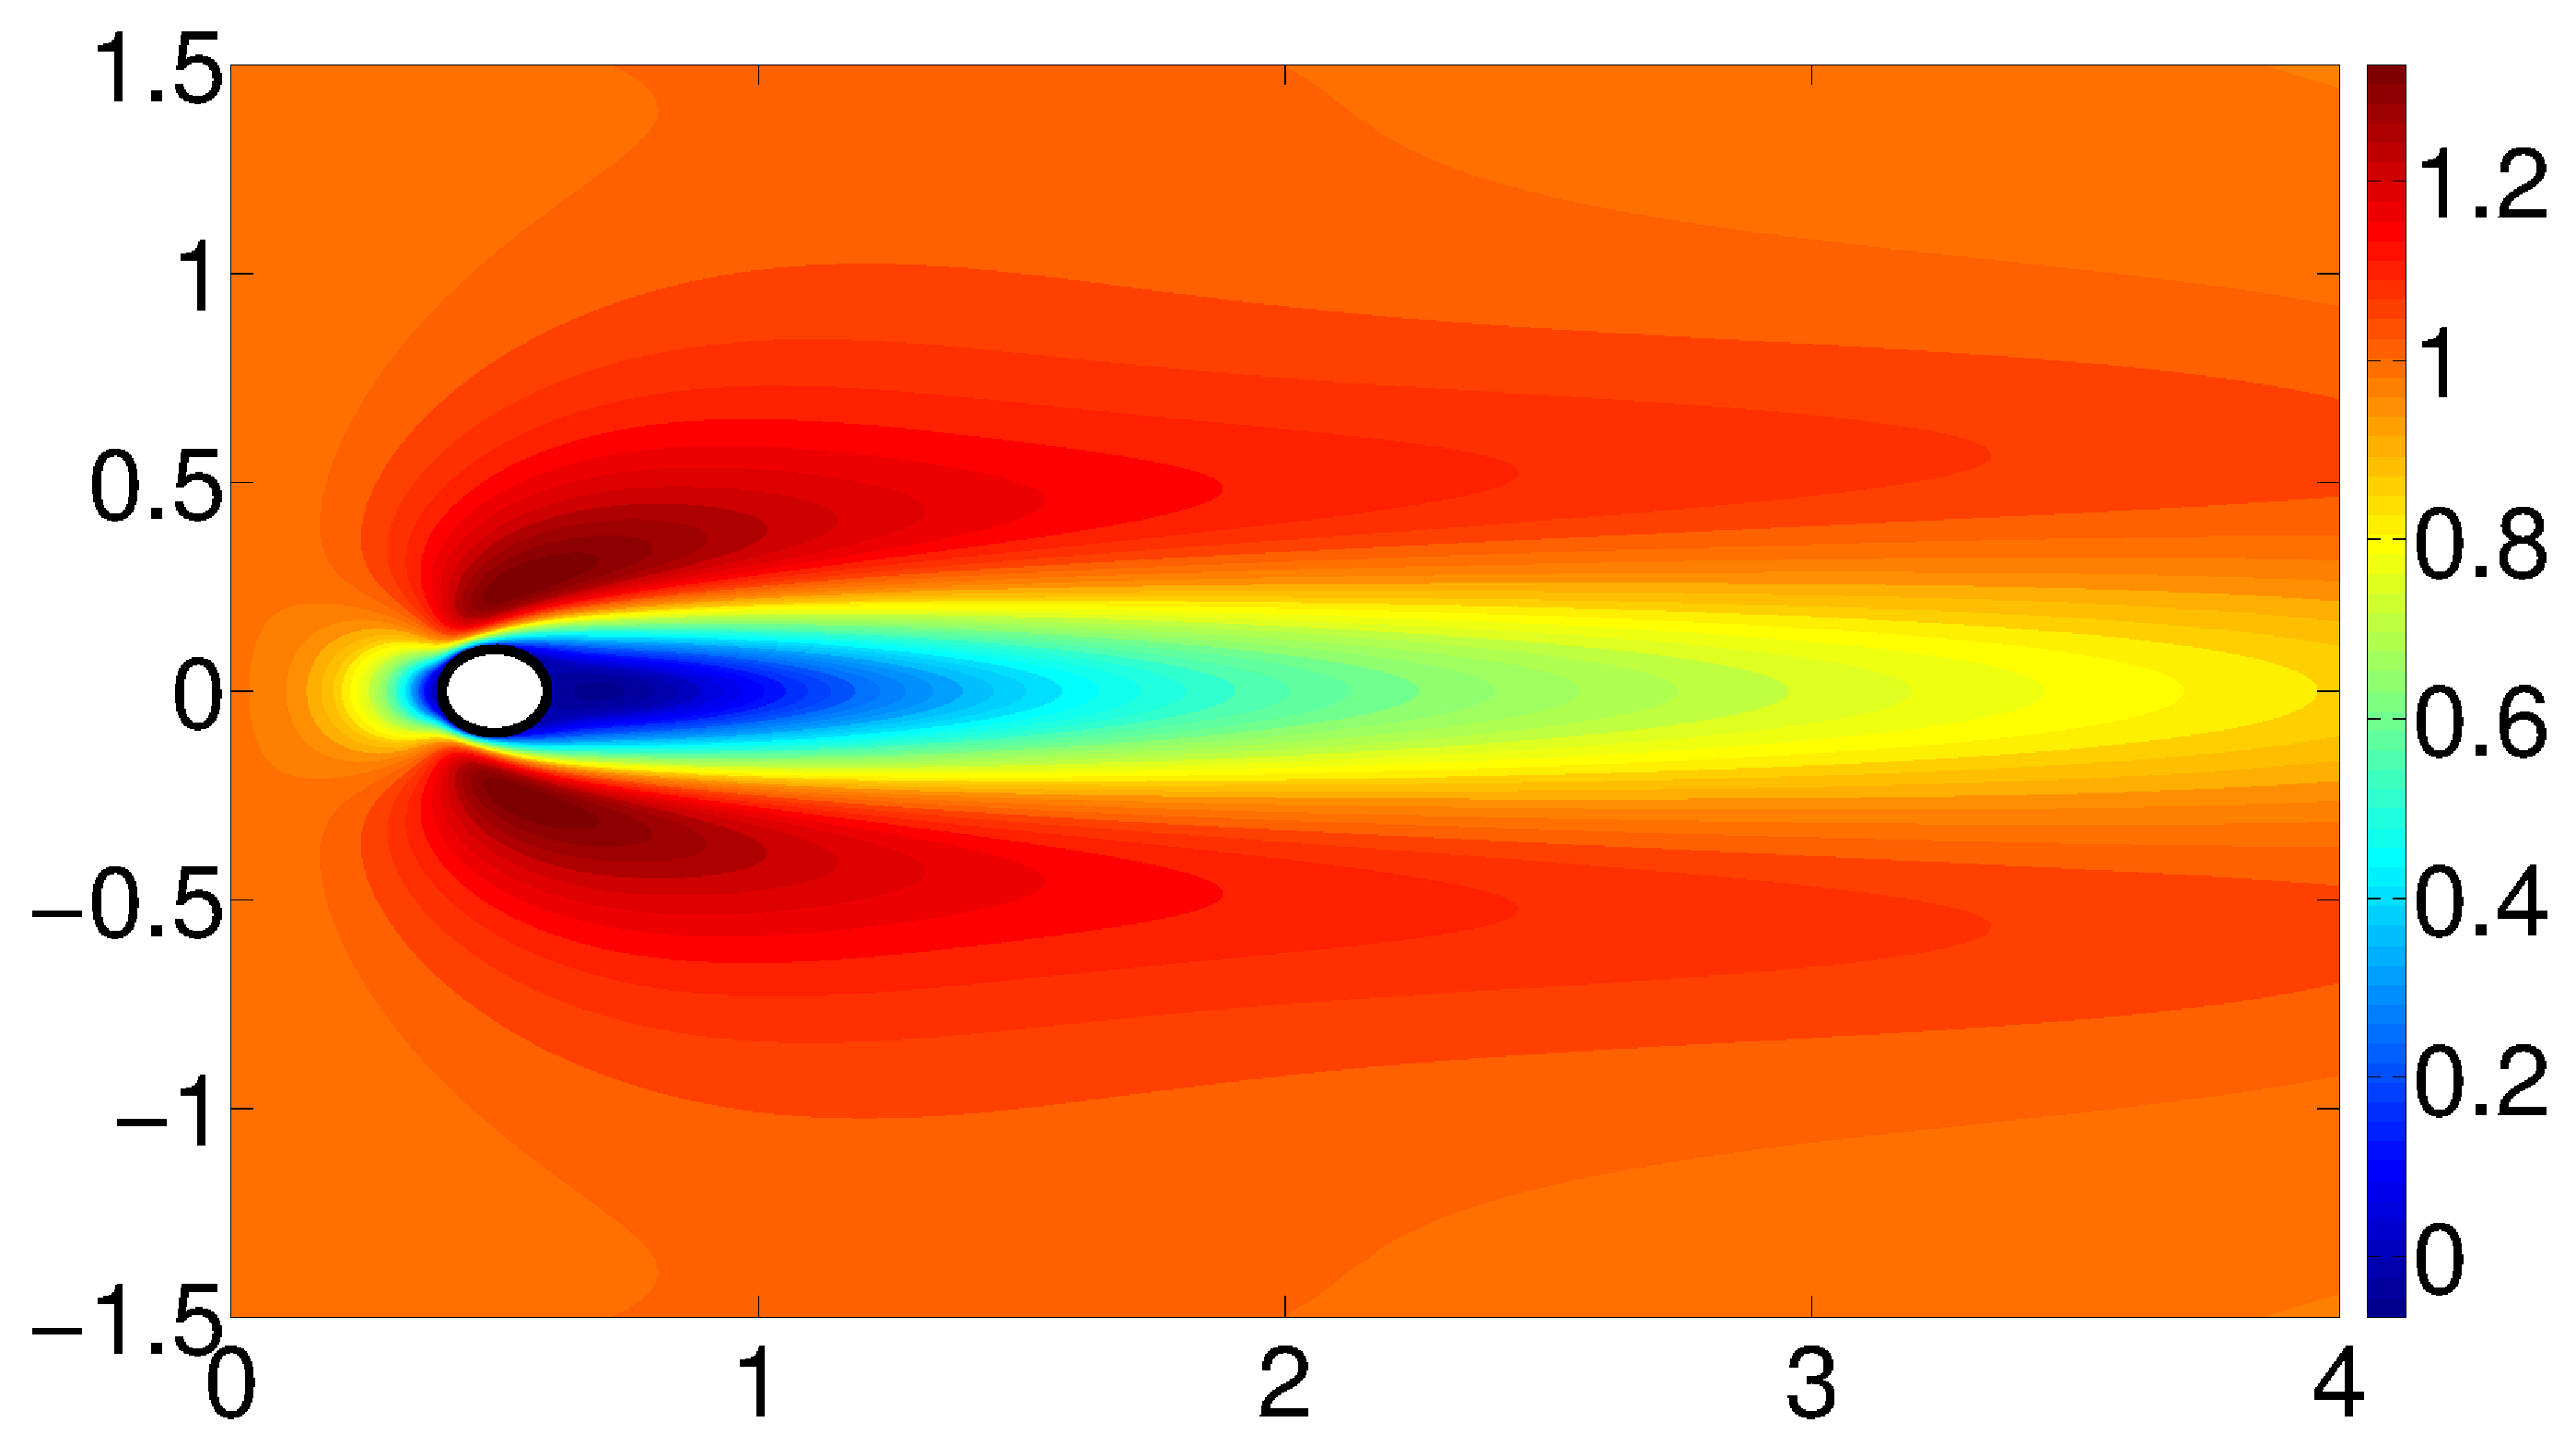
\includegraphics[width=7.0cm]{Chapter_4/figure/flow_over_cylinder/u_velocity_contour_RE100.eps}
    }
    \quad
    \subfigure[V-velocity]
    {
    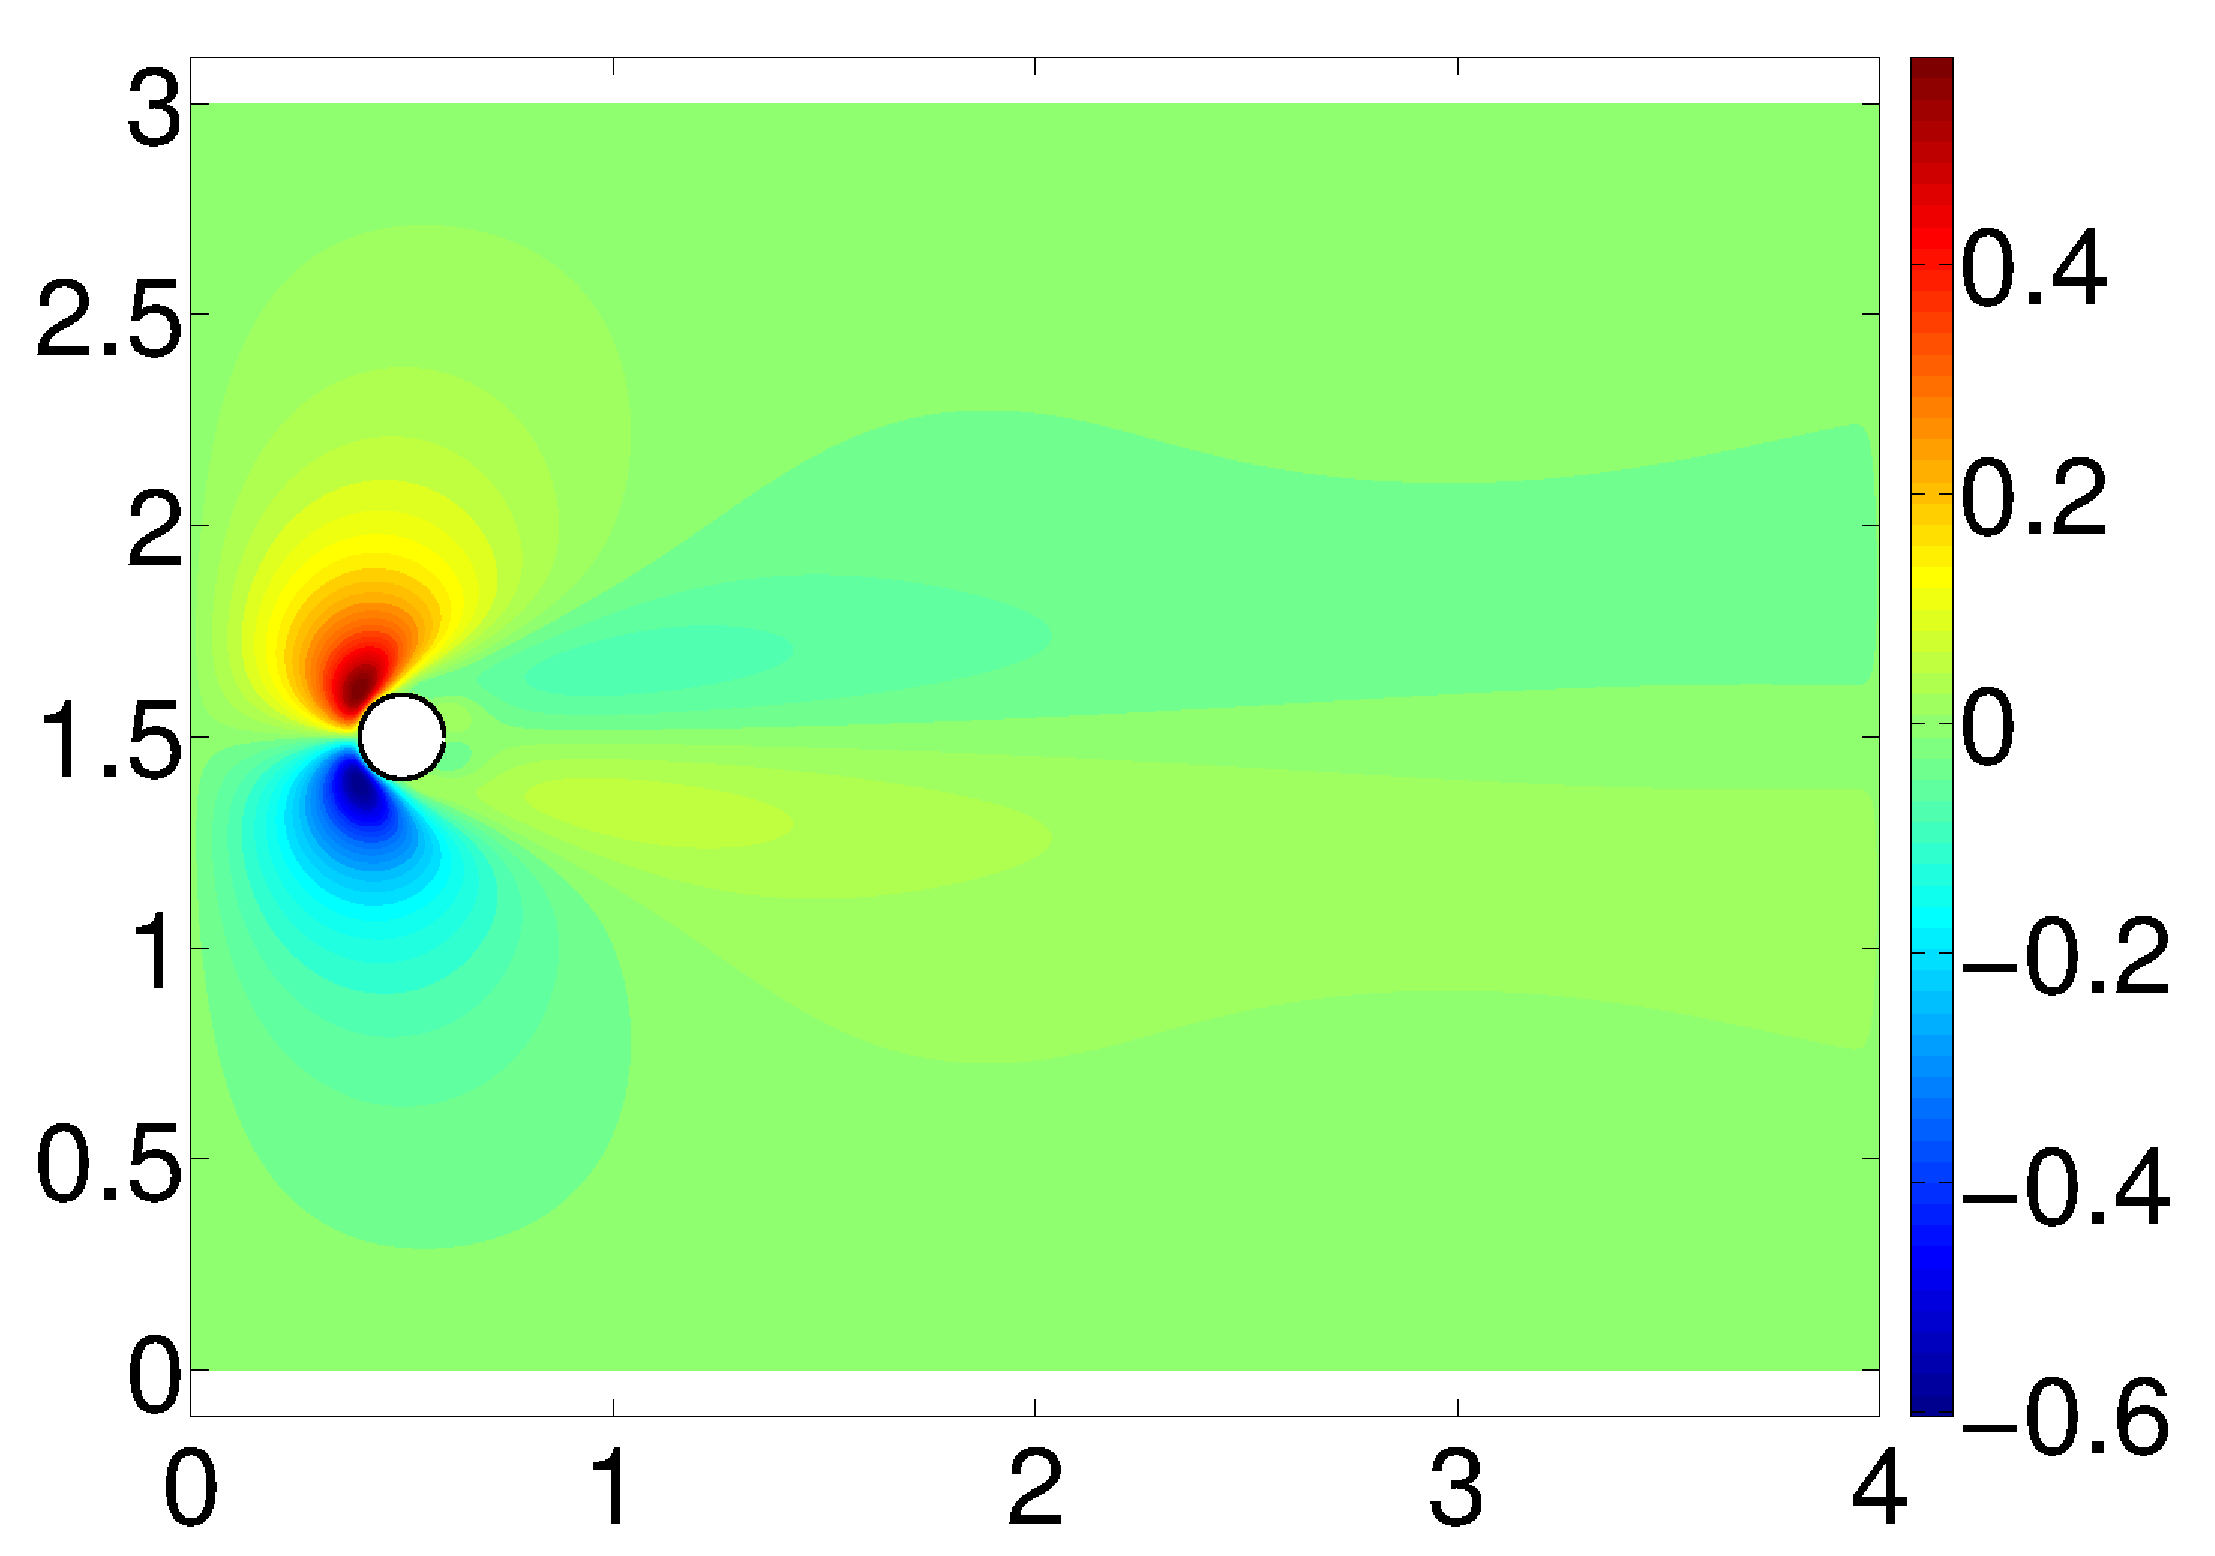
\includegraphics[width=7.0cm]{Chapter_4/figure/flow_over_cylinder/v_velocity_contour_RE100.eps}
    }
    \caption{Velocity contours for Re = 100.}
    \label{fig:contourPlotsForFlowOverCylidnerGE}
\end{figure}

To ensure that the zero velocity on the solid boundary, we looked at the value of the u and v velocities at the Lagrangian points on the boundary.